\chapter{\#3: Potts model on arbitrary topologies}

\resp{Robin Chan}

%\emph{
%Structure as\footnote{Remove this part from the report}:
%\begin{itemize}
%\item A short (max 1 page) explanation of the task, including references. Include mathematical concepts.
%\item Max 2 pages for the whole task (including figures)
%\item It is possible to use appendices for supplementary material, at the end of the report. Max 5 pages per task
%\end{itemize}
%A total of 3 pages + 5 supplementary pages per task
%}

\section{Introduction}
 
The Potts model forms a natural extension to the Ising model. Instead of looking at model where every element can have one of two values (\textit{up} or \textit{down}), the Potts model has $p$ possible states. The Ising model is most well-known for its application to lattices, however, this task will analyse the behaviour of the Potts model on arbitrary topologies. This project is based on a paper by Dorogovtsev et al. \cite{pottspaper} and a review paper by Dorogovtsev et al. \cite{pottsreview}.

To generate an arbitrary network, the configuration model is used where the degree distribution is parametrised as a power law $P(k) \propto k^{-\gamma}$. The Hamiltonian of this Potts model is given by:

\begin{equation}
    H = -J \sum_{<ij>} \delta_{\alpha_i, \alpha_j} - H \sum_i \delta_{\alpha_i, 1}
\end{equation}

\noindent where the first sum goes over all edges and the second over all vertices. $\alpha_i$ refers to the state of node $i$ ($\alpha_i = (1, ..., p)$). This project will work with $J = 1$ and $H = 0$.

To simulate this system the Metropolis Hastings Monte Carlo algorithm was used. The network starts off as a random realisation of the configuration model with random ''spins'' (running from 1 to $p$) assigned to each node. At each time step a random node is assigned a new random spin. The energy of the system is then computed. If this action has lowered the energy, the new configuration is accepted. If it does not lower the energy, the new configuration is accepted with probability $e^{-\frac{\Delta E}{kT}}$. This helps to prevent getting stuck in local minima while still sampling in a directed manner (i.e. not exploring the phase space at random).

\section{Results}
All simulations were run on a network of 500 nodes.
Let us first perform a sanity check. Does the implemented MHMC algorithm actually minimise the energy? For this the procedure is repeated 10 times for random realisations of the network. All quantities are then averaged out over these 10 iterations, resulting in Fig. \ref{potts energy evol}.

\begin{figure}[H]
    \centering
    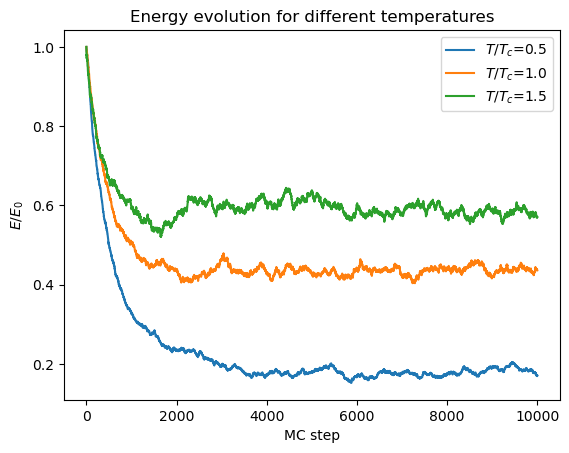
\includegraphics[width=0.7\linewidth]{images/potts_energy evol.png}
    \caption{\textit{Energy evolution of the Potts model for different temperatures}}
    \label{potts energy evol}
\end{figure}

The energy can be seen levelling off and an increase of the equilibrium energy and its fluctuations is seen for higher temperatures. This is the expected behaviour for this system indicating that our algorithm is implemented correctly.

Trying to reproduce the critical behaviour of this system resulted in some strange results. When looking at the magnetisation of the system as a function of the temperature, no clear result could be obtained. I am still not sure why. The paper's definition for the average magnetisation is used, but I am unable to interpret the result in Figure \ref{avmag}.

\begin{figure}[H]
    \centering
    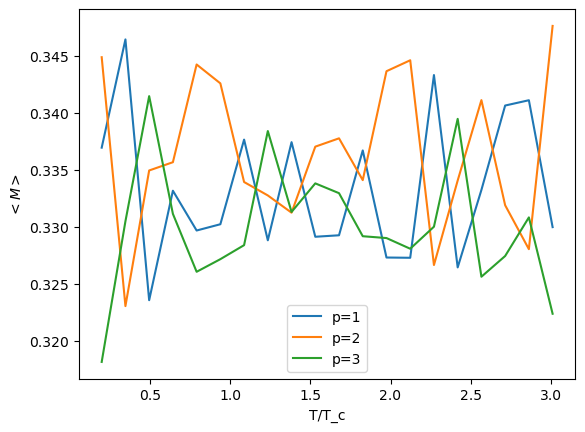
\includegraphics[width=0.5\linewidth]{images/av_mag.png}
    \caption{\textit{Average magnetisation for a three state Potts model}}
    \label{avmag}
\end{figure}

\newpage